\documentclass[pdflatex,compress]{beamer}

%\usetheme[dark,framenumber,totalframenumber]{ElektroITK}
\usetheme[darktitle,framenumber,totalframenumber]{ElektroITK}

\usepackage{graphicx}

\title{PEMODELAN JARINGAN KOMUNIKASI}
\subtitle{Host to Host Communications}

\author{Mifta Nur Farid, S.T., M.T.}

\begin{document}

\maketitle

\section{Cisco Operating Systems}

\begin{frame}
	\frametitle{A Short History of Cisco Operating Systems}
	\begin{itemize}
		\item Most people think of Cisco as primarily a routing and switching company, but they actually started out with just routers in 1984.
		\item IOS is the operating system that has been used on Cisco routers since their inception.
		\item Cisco Catalyst switches evolved from the acquisition of Crescendo in 1993.
		\item The original Cisco switch operating system was CatOS, which has now been deprecated.
	\end{itemize}
\end{frame}

\begin{frame}
	\frametitle{A Short History of Cisco Operating Systems}
	\begin{itemize}
		\item Cisco firewalls evolved from the acquisition of Network Translation’s PIX firewall with Finesse operating system in 1995.
		\item Cisco switches and firewalls were ported over to the IOS operating system over the following years.
	\end{itemize}
\end{frame}

\begin{frame}
	\frametitle{Other Cisco Operating Systems}
	\begin{itemize}
		\item IOS remains as the operating system used on the majority of Cisco enterprise grade network devices.
		\item Other operating systems have been developed for some more recent router and switch platforms.
	\end{itemize}
\end{frame}

\begin{frame}
	\frametitle{Other Cisco Operating Systems}
	\begin{itemize}
		\item The Cisco Nexus and MDS data center switch product lines run on \textbf{NX-OS}.
		\item The \textbf{IOS-XR} operating system runs on the service provider NCS, CRS, ASR9000 and XR12000 series routers.
		\item \textbf{IOS-XE} runs on the ASR1000 series service provider routers.
		\item The Command Line Interfaces for the other operating systems are nearly identical to IOS.
	\end{itemize}
\end{frame}


\section{Connecting to a Cisco Device over the network}

\begin{frame}
	\frametitle{Connecting to a Cisco Device over the network}
	\begin{itemize}
		\item The lab exercises in this course use Cisco Packet Tracer simulation software on your PC.
		\item This lecture shows how to connect to a real router or switch over the network with Putty.
		\item You do not need to install or use Putty to do the course lab exercises.
	\end{itemize}
\end{frame}

\begin{frame}
	\frametitle{Connecting over the network}
	\begin{center}
		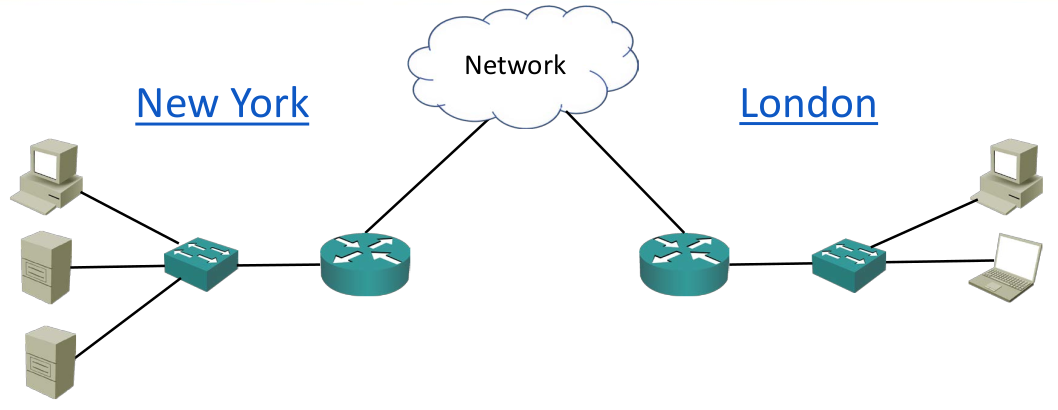
\includegraphics[width=1\linewidth]{img/img01}
	\end{center}
\end{frame}

\begin{frame}
	\frametitle{Connecting to a Cisco Device}
	\begin{itemize}
		\item To get to the Command Line Interface for day to day management of a Cisco device you will use Secure Shell (SSH) to connect to it’s management IP address over the network.
		\item Telnet is also supported but not recommended because it is insecure.
		\item In enterprise networks, secure login will typically be enforced through integration with a centralised AAA (Authentication, Authorization and Accounting) server.
		\item We will cover SSH and AAA in later lessons.
	\end{itemize}
\end{frame}

\begin{frame}
	\frametitle{Out of Band Management}
	\begin{center}
		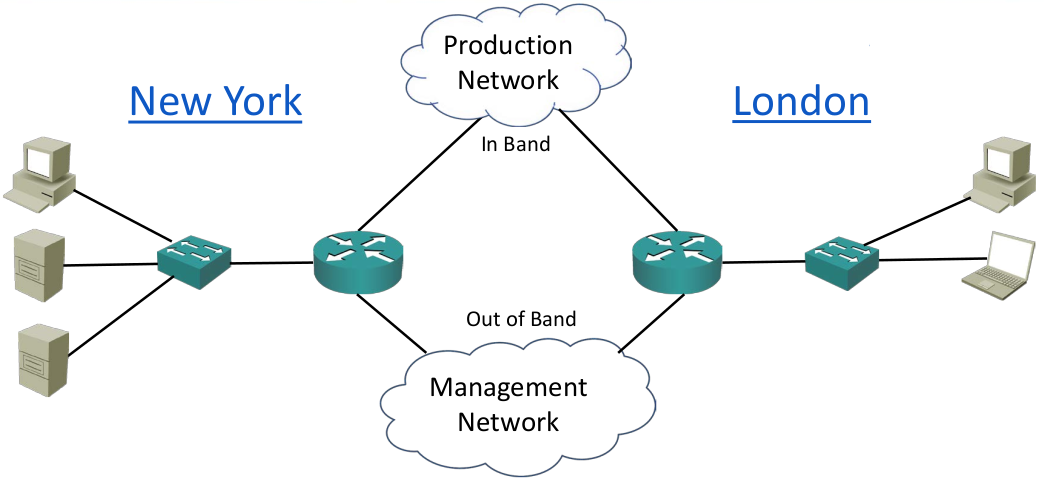
\includegraphics[width=1\linewidth]{img/img02}
	\end{center}
\end{frame}

\section{Initial Connection to a Cisco Device}

\begin{frame}
	\frametitle{Connecting to a Cisco Device}
	\begin{itemize}
		\item This lecture shows how to connect to a real router or switch over a console connection with Putty.
		\item The lab exercises in this course use Cisco Packet Tracer simulation software on your PC.
		\item You do not need to install or use Putty to do the course lab exercises.
		\item See Section 2 ‘How to Set Up the Lab’ for step by step instructions on how to use Packet Tracer for the course lab exercises.
	\end{itemize}
\end{frame}

\begin{frame}
	\frametitle{Initial Connection to a Cisco Device}
	\begin{itemize}
		\item Cisco devices do not usually have a default IP address, so we need to set one up before we can connect to it over the network.
		\item We need a way to connect to the device to do the initial configuration including adding IP addresses. This is where the console connection comes in.
	\end{itemize}
\end{frame}

\begin{frame}
	\frametitle{The Console Cable (DB9 to RJ45)}
	\begin{center}
		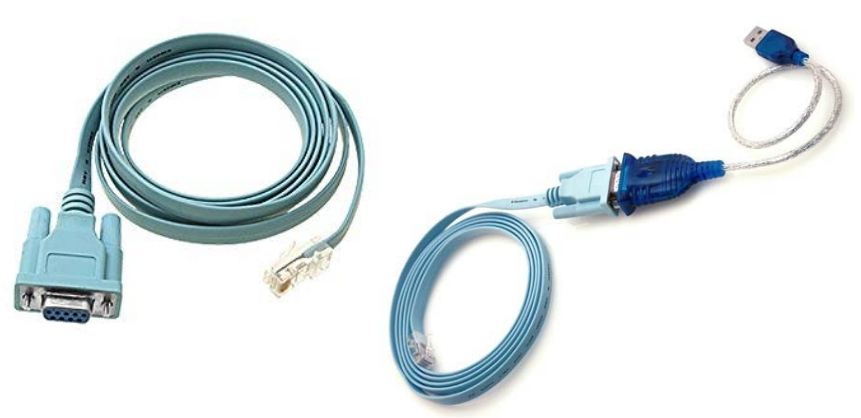
\includegraphics[width=1\linewidth]{img/img03}
	\end{center}
\end{frame}

\begin{frame}
	\frametitle{The New Console Cable (USB to Mini-USB)}
	\begin{center}
		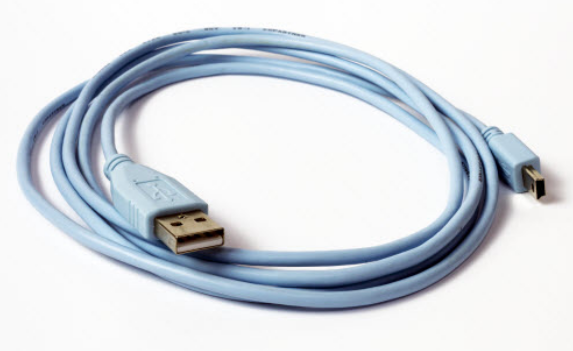
\includegraphics[width=1\linewidth]{img/img04}
	\end{center}
\end{frame}

\begin{frame}
	\frametitle{Console Connection Troubleshooting}
	\begin{itemize}
		\item As well as for initial configuration, the console port can be used if the device’s IP addresses become unresponsive.
		\item It can also be used to troubleshoot the bootup process. You can view the device booting up from a console connection but this is not possible with SSH because the system must have booted already before the IP address will be live.
	\end{itemize}
\end{frame}

\section{Navigating the Cisco IOS Operating System}

\begin{frame}
	\frametitle{IOS Command Hierarchy}
	\begin{itemize}
		\item hostname$ > $ $\rightarrow$ User Exec mode
		\item hostname$ \# $ $\rightarrow$ Privileged Exec mode ('Enable')
		\item hostname(config)$ \# $ $\rightarrow$ Global Configuration mode ('Configure Terminal')
		\item hostname(config-if)$ \# $ $\rightarrow$ Interface Configuration mode ('Interface x')
		\item 'Exit' drops back down a level.
		\item 'End' drops back to Privileged Exec mode from any level.
	\end{itemize}
\end{frame}

\begin{frame}
	\frametitle{Command Abbreviation}
	\begin{itemize}
		\item You can type in a shortened version of a command.
		\item For example, 'en' instead of 'enable'
		\item There must be only one possible match for what you typed for abbreviation to succeed
	\end{itemize}
\end{frame}

\begin{frame}
	\frametitle{Context Sensitive Help}
	\begin{itemize}
		\item You can enter a question mark to access Help
		\item ‘sh?’ will show all commands that begin with ‘sh’
		\item ‘show ?’ will show all available keyword options for the ‘show’ command
		\item ‘show ip ?’ will show all available keyword options for the ‘show ip command’
	\end{itemize}
\end{frame}

\begin{frame}
	\frametitle{Moving the Cursor}
	\begin{itemize}
		\item Backspace deletes the previous character
		\item The arrow keys ( $ < $ and $ > $ ) move the cursor left and right one character at a time
		\item Ctrl-A moves the cursor to the beginning of the line
		\item Ctrl-U deletes the whole line
		\item See http://etherealmind.com/cisco-ios-cli-shortcuts/ for more
	\end{itemize}
\end{frame}

\begin{frame}
	\frametitle{Command History}
	\begin{itemize}
		\item The up and down arrows ( $\downarrow$ and $\uparrow$ ) cycle through previously entered commands at the same level in the hierarchy.
	\end{itemize}
\end{frame}

\begin{frame}
	\frametitle{Showing command output}
	\begin{itemize}
		\item Enter will show ‘show’ command output which scrolls off the end of the page line by line.
		\item The Spacebar will show it page by page.
		\item Ctrl-C will break out of the show command output and return to the command prompt.
	\end{itemize}
\end{frame}

\begin{frame}
	\frametitle{Piped Command Examples}
	\begin{itemize}
		\item show running-config interface FastEthernet0/0
		\item show running-config $ | $ begin FastEthernet0/0
		\item show running-config $ | $ include FastEthernet0/0
		\item show running-config $ | $ exclude FastEthernet0/0
		\item show running-config $ | $ section interface
	\end{itemize}
\end{frame}

\begin{frame}
	\frametitle{Configuration Storage Locations}
	\begin{itemize}
		\item The IOS operating system image is stored in Flash.
		\item The Startup Configuration is stored in NVRAM.
		\item The Running Configuration is stored in RAM. (Loaded into RAM from the Startup Config when the device boots up.)
	\end{itemize}
\end{frame}

\begin{frame}
	\frametitle{Saving the Configuration}
	\begin{itemize}
		\item Commands take effect immediately but are not persistent across a reboot.
		\item Enter ‘copy running-config startup-config’ to make the configuration persistent.
		\item Enter ‘wr erase’ or ‘erase startup-config’ and then ‘reload’ to delete the starting configuration and factory reset the device.
	\end{itemize}
\end{frame}

\begin{frame}
	\begin{center}
		
\includegraphics[width=1\linewidth]{../../img/thank_you}
	\end{center}
\end{frame}

\begin{frame}
	\begin{center}
		
\includegraphics[width=1\linewidth]{../../img/any_questions}
	\end{center}
\end{frame}

\end{document}